% tugas_data_analitik.tex
% Laporan Tugas Data Analitik — C-MAPSS RUL Prediction (Complete Version)
% Departemen Teknik Mesin FTUI — 2026

\documentclass[11pt,a4paper]{article}

\usepackage[T1]{fontenc}
\usepackage[utf8]{inputenc}
\usepackage[a4paper, margin=2.5cm]{geometry}
\usepackage{setspace}
\usepackage{parskip}
\usepackage{titlesec}
\usepackage{fancyhdr}
\usepackage{booktabs}
\usepackage{tabularx}
\usepackage{multirow}
\usepackage{graphicx}
\usepackage{caption}
\usepackage{subcaption}
\usepackage{xcolor}
\usepackage{amsmath}
\usepackage{amssymb}
\usepackage{hyperref}
\usepackage{enumitem}
\usepackage{float}
\usepackage{tocloft}
\usepackage{url}

\definecolor{uiblue}{RGB}{0,56,147}
\definecolor{mygray}{RGB}{100,100,100}
\definecolor{matgreen}{RGB}{0,120,0}

\titleformat{\section}
  {\large\bfseries\color{uiblue}}
  {\thesection}{0.6em}{}[\vspace{2pt}\hrule\vspace{4pt}]
\titleformat{\subsection}
  {\normalsize\bfseries\color{uiblue}}{\thesubsection}{0.6em}{}
\titleformat{\subsubsection}
  {\small\bfseries}{\thesubsubsection}{0.6em}{}

\pagestyle{fancy}
\fancyhf{}
\fancyhead[L]{\small\color{mygray}
  Tugas Data Analitik -- Prediksi RUL Mesin Turbofan C-MAPSS}
\fancyhead[R]{\small\color{mygray} Data Analitik 2026}
\fancyfoot[C]{\small\color{mygray}\thepage}
\renewcommand{\headrulewidth}{0.4pt}
\renewcommand{\footrulewidth}{0.0pt}

\onehalfspacing
\captionsetup{font=small, labelfont=bf}
\hypersetup{colorlinks=true, linkcolor=uiblue,
            urlcolor=uiblue, citecolor=uiblue}

% ══════════════════════════════════════════════════════════════════════════════
\begin{document}

% ── Cover ─────────────────────────────────────────────────────────────────────
\begin{titlepage}
  \centering
  \vspace*{1.0cm}
  
\includegraphics[width=2.2cm]{images/logo_ui.png}
  \vspace{0.6cm}

  {\large\bfseries UNIVERSITAS INDONESIA\par}
  \vspace{0.2cm}
  {\normalsize Fakultas Teknik -- Departemen Teknik Mesin\par}

  \vspace{0.5cm}
  \hrule height 1.2pt
  \vspace{0.4cm}
  {\LARGE\bfseries\color{uiblue}
    PREDIKSI \textit{REMAINING USEFUL LIFE}\\[0.3em]
    MESIN TURBOFAN MENGGUNAKAN\\[0.3em]
    \textit{ARTIFICIAL NEURAL NETWORK}\\[0.3em]
    PADA DATASET C-MAPSS\par}
  \vspace{0.4cm}
  \hrule height 1.2pt

  \vspace{1.0cm}
  {\normalsize\color{mygray} Mata Kuliah:\par}
  {\large\bfseries Data Analitik\par}
  \vspace{0.6cm}
  {\normalsize\color{mygray} Dosen Pengampu:\par}
  {\normalsize Dr.\ Eng.\ Sholahudin, S.T., M.Sc.\par}

  \vspace{0.8cm}
  {\normalsize\color{mygray} Disusun Oleh:\par}
  \vspace{0.4cm}
  \begin{tabular}{ll}
    2506565466 & Luqman Alifio Arhab \\[4pt]
    2506565414 & Azfa Rhazasta Abiandra \\[4pt]
    2506565401 & Adamsyah Haryo Saksono \\[4pt]
    2506565433 & Epsiarto Rizqi Nurwijayadi \\[4pt]
  \end{tabular}

  \vspace{0.2cm}
  \vfill
  {\normalsize\bfseries
    DEPARTEMEN TEKNIK MESIN\\
    FAKULTAS TEKNIK\\
    UNIVERSITAS INDONESIA\\[0.4em]
    2026\par}
\end{titlepage}

\thispagestyle{empty}
\newpage
\setcounter{page}{1}
\tableofcontents
\newpage

% ══════════════════════════════════════════════════════════════════════════════
\section{Pendahuluan}

\subsection{Latar Belakang}

Prediksi \textit{Remaining Useful Life} (RUL) merupakan komponen kunci dalam
sistem \textit{Prognostics and Health Management} (PHM). Dengan mengetahui
sisa umur pakai komponen sebelum kegagalan, jadwal perawatan dapat
dioptimalkan sehingga mengurangi biaya \textit{downtime} tak terencana.

\begin{figure}[H]
  \centering
  
\includegraphics[width=0.58\textwidth]{images/01_phm_ecosystem_stack.png}
  \caption{Hierarki PHM --- laporan ini berfokus pada lapisan
    \textit{Prognostics} (prediksi RUL)}
  \label{fig:phm}
\end{figure}

\subsection{Tujuan}

\begin{enumerate}[noitemsep]
  \item Membersihkan data dengan analisis korelasi sensor terhadap output (RUL)
  \item Menormalisasi data dengan \textit{z-score} berbasis siklus sehat
  \item Memilih fitur menggunakan korelasi Pearson dan PCA
  \item Membangun model MLP pada empat sub-dataset dengan dua implementasi:
    Python (PyTorch) dan MATLAB (feedforwardnet)
  \item Menganalisis kepentingan fitur dengan algoritma Garson
  \item Membandingkan hasil kedua implementasi
\end{enumerate}

\subsection{Alur Pipeline}

\begin{figure}[H]
  \centering\small
  \begin{tabular}{ccccc}
    \fbox{Raw .txt NASA} & $\rightarrow$ &
    \fbox{HDF5 / CSV} & $\rightarrow$ &
    \fbox{Cleaning} \\[6pt]
    & & & & $\downarrow$ \\[2pt]
    \fbox{Garson} & $\leftarrow$ &
    \fbox{ANN (Python + MATLAB)} & $\leftarrow$ &
    \fbox{Normalisasi + PCA}
  \end{tabular}
  \caption{Alur pipeline analitik --- diimplementasikan di Python dan MATLAB}
  \label{fig:pipeline}
\end{figure}

% ══════════════════════════════════════════════════════════════════════════════
\section{Dataset C-MAPSS}

\subsection{Deskripsi Dataset}

Dataset C-MAPSS dipublikasikan oleh NASA \cite{saxena2008}:
\begin{center}
  \small\url{https://www.nasa.gov/intelligent-systems-division/discovery-and-systems-health/pcoe/pcoe-data-set-repository/}
\end{center}

\begin{figure}[H]
  \centering
  
\includegraphics[width=0.90\textwidth]{images/09_dataset_matrix.png}
  \caption{Matriks karakteristik empat sub-dataset C-MAPSS}
  \label{fig:dataset_matrix}
\end{figure}

\begin{figure}[H]
  \centering
  
\includegraphics[width=0.88\textwidth]{images/03_cmapss_engine_schematic.png}
  \caption{Skema mesin turbofan C-MAPSS --- 21 sensor mengukur kondisi
    sepanjang aliran udara; HPC adalah komponen yang terdegradasi}
  \label{fig:engine}
\end{figure}

\subsection{Konsep RUL dan Struktur File}

\begin{figure}[H]
  \centering
  
\includegraphics[width=0.85\textwidth]{images/10_train_test_rul_relationship.png}
  \caption{Hubungan antara file train, test, dan RUL}
  \label{fig:rul_rel}
\end{figure}

\subsection{Motivasi: Mengapa RUL Sulit Diprediksi}

\begin{figure}[H]
  \centering
  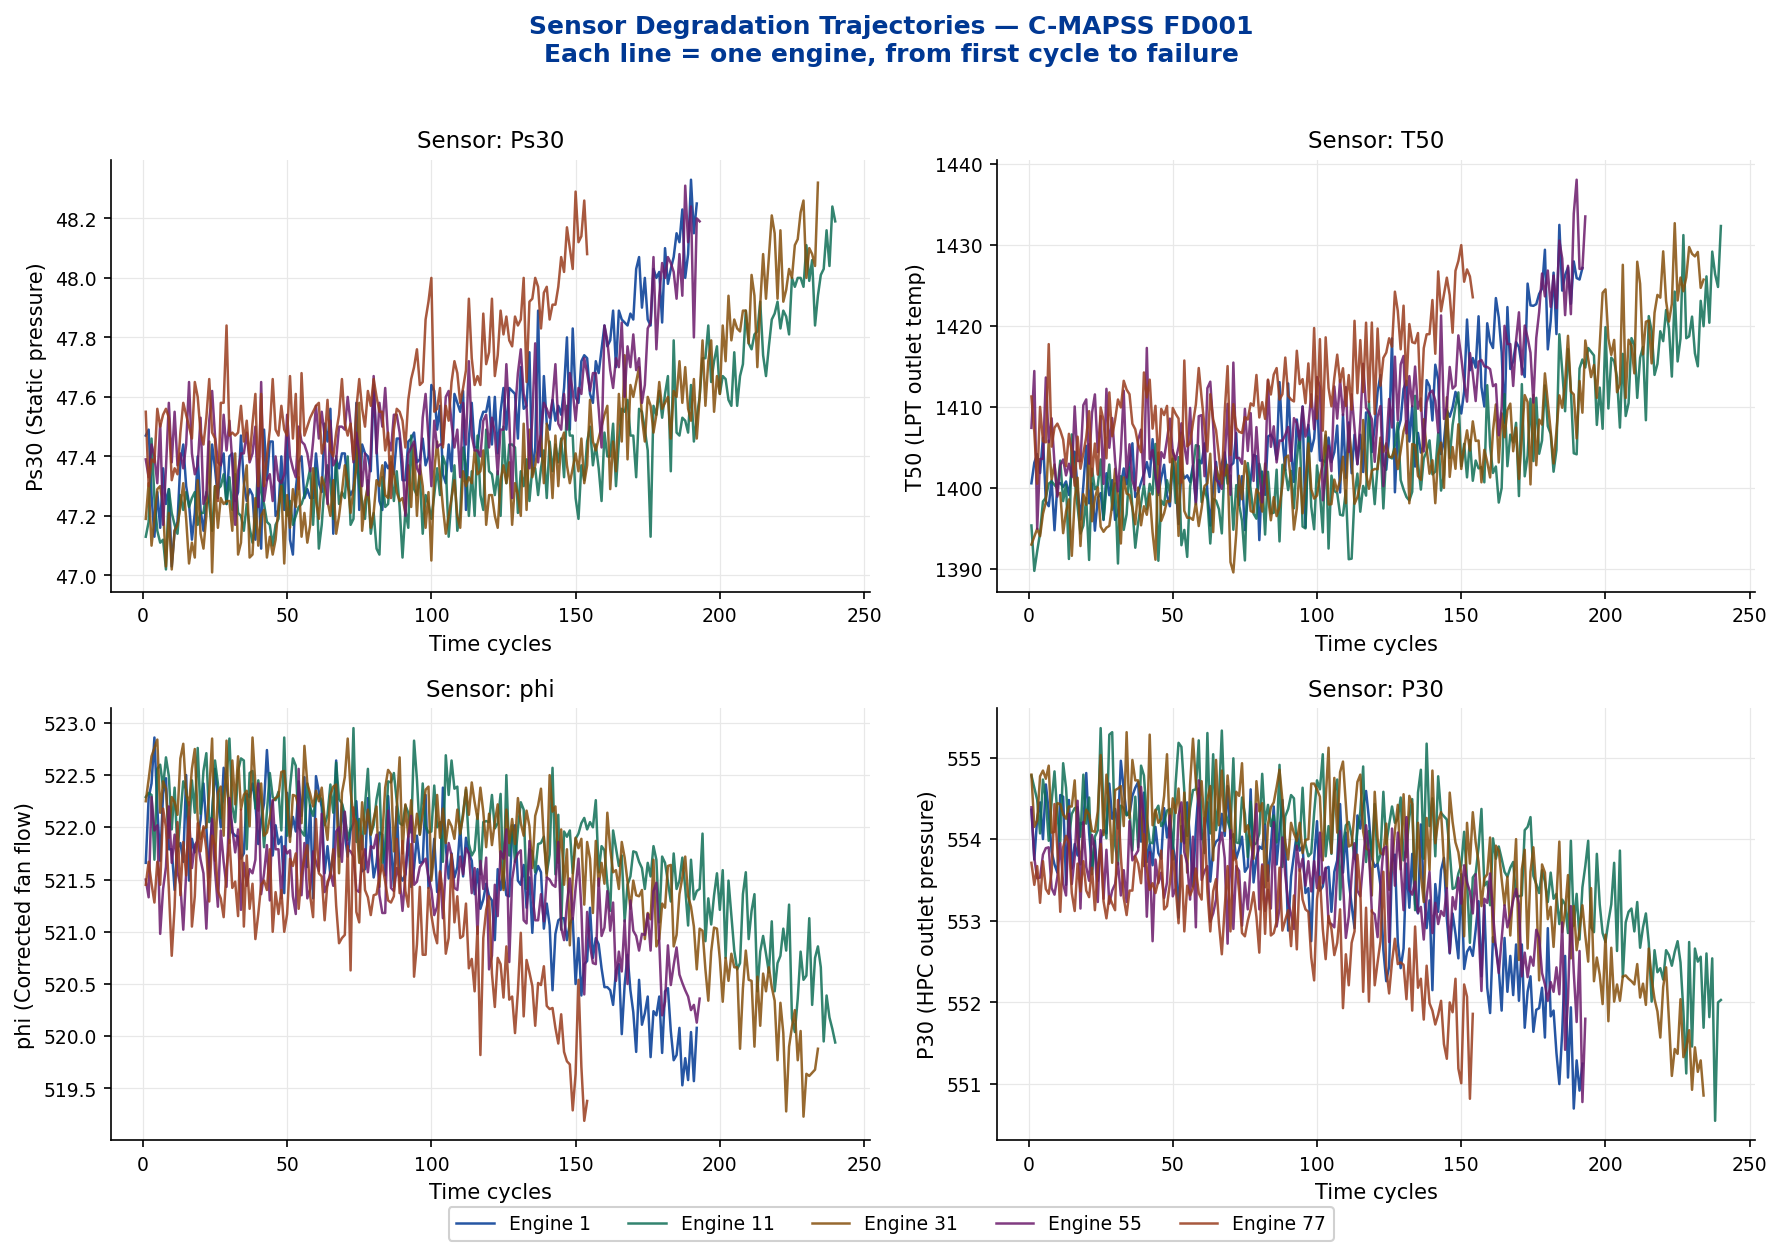
\includegraphics[width=0.95\textwidth]{images/plot_A1_degradation.png}
  \caption{Trajektori degradasi sensor FD001 untuk lima mesin ---
    sensor Ps30, T50, phi, P30 menunjukkan \textit{drift} menjelang
    akhir umur mesin (Python)}
  \label{fig:degradation_py}
\end{figure}

\begin{figure}[H]
  \centering
  
\includegraphics[width=0.95\textwidth]{images/matlab_A1_degradation.png}
  \caption{Trajektori degradasi sensor FD001 --- implementasi MATLAB}
  \label{fig:degradation_mat}
\end{figure}

\subsection{Struktur HDF5}

\begin{figure}[H]
  \centering
  \begin{subfigure}[b]{0.30\textwidth}
    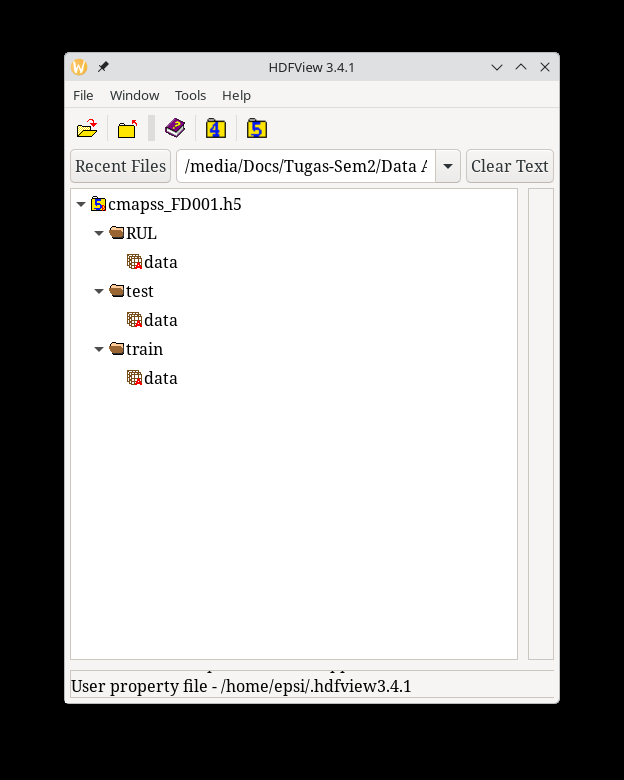
\includegraphics[width=\textwidth]{images/hdf5-01-vanilla-01-main.png}
    \caption{Vanilla}
  \end{subfigure}
  \hfill
  \begin{subfigure}[b]{0.30\textwidth}
    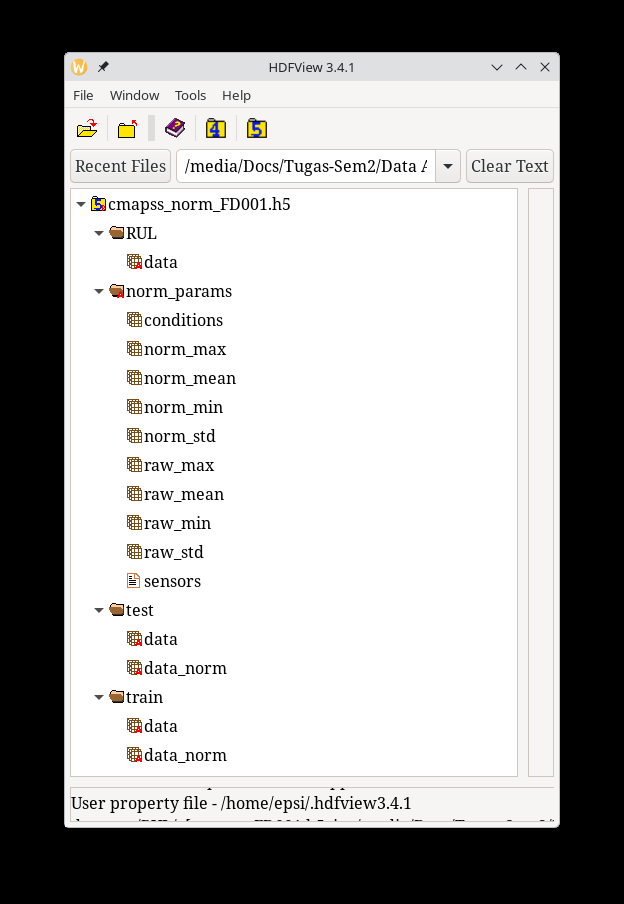
\includegraphics[width=\textwidth]{images/hdf5-03-normal-01-main.png}
    \caption{+ Normalisasi}
  \end{subfigure}
  \hfill
  \begin{subfigure}[b]{0.30\textwidth}
    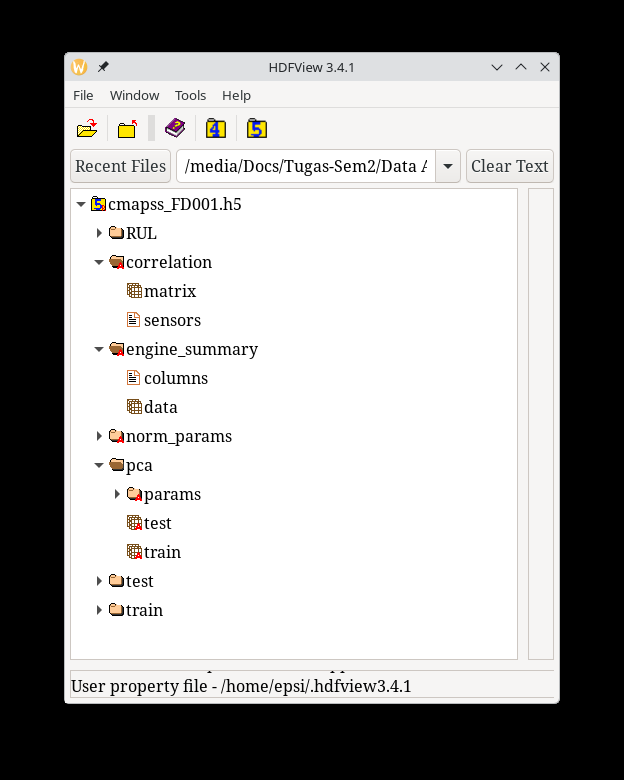
\includegraphics[width=\textwidth]{images/hdf5-05-pca-01-main.png}
    \caption{+ Korelasi + PCA}
  \end{subfigure}
  \caption{Evolusi struktur HDF5 dari vanilla hingga lengkap}
  \label{fig:hdf5}
\end{figure}

% ══════════════════════════════════════════════════════════════════════════════
\section{Pembersihan Data}

\subsection{Metode}

Lima metode statistik digunakan untuk menganalisis korelasi sensor
terhadap output (RUL):
std, CV, Pearson vs RUL, Spearman vs RUL, dan Mutual Information vs RUL.

\subsection{Hasil Analisis FD001}

\begin{table}[H]
\centering\small
\caption{Statistik sensor FD001 terhadap output RUL}
\label{tab:sensor_stats}
\begin{tabular}{lrrrrrrl}
\toprule
Sensor & Mean & Std & CV & Pearson & Spearman & MI & Hapus \\
\midrule
T2$^\dagger$         & 518.67 & 0.000 & 0.000 & NaN     & NaN     & 0.000 & \checkmark \\
T24          & 642.68 & 0.500 & 0.001 & $-$0.607 & $-$0.629 & 0.342 & \\
T30          & 1590.5 & 6.131 & 0.004 & $-$0.585 & $-$0.606 & 0.306 & \\
T50          & 1408.9 & 9.001 & 0.006 & $-$0.679 & $-$0.702 & 0.467 & \\
P2$^\dagger$         &  14.62 & 0.000 & 0.000 & NaN     & NaN     & 0.006 & \checkmark \\
P15          &  21.61 & 0.001 & 0.000 & $-$0.128 & $-$0.128 & 0.006 & \checkmark \\
P30          & 553.37 & 0.885 & 0.002 & $+$0.657 & $+$0.679 & 0.425 & \\
Nf           & 2388.1 & 0.071 & 0.000 & $-$0.564 & $-$0.574 & 0.258 & \\
Nc           & 9065.2 & 22.08 & 0.002 & $-$0.390 & $-$0.322 & 0.222 & \\
epr$^\dagger$        &   1.30 & 0.000 & 0.000 & NaN     & NaN     & 0.000 & \checkmark \\
Ps30         &  47.54 & 0.267 & 0.006 & $-$0.696 & $-$0.718 & 0.507 & \\
phi          & 521.41 & 0.738 & 0.001 & $+$0.672 & $+$0.693 & 0.442 & \\
NRf          & 2388.1 & 0.072 & 0.000 & $-$0.563 & $-$0.573 & 0.262 & \\
NRc          & 8143.8 & 19.08 & 0.002 & $-$0.307 & $-$0.202 & 0.225 & \\
BPR          &   8.44 & 0.038 & 0.004 & $-$0.643 & $-$0.666 & 0.390 & \\
farB$^\dagger$       &   0.03 & 0.000 & 0.000 & NaN     & NaN     & 0.000 & \checkmark \\
htBleed      & 393.21 & 1.549 & 0.004 & $-$0.606 & $-$0.629 & 0.328 & \\
Nf\_dmd$^\dagger$    & 2388.0 & 0.000 & 0.000 & NaN     & NaN     & 0.000 & \checkmark \\
PCNfR\_dmd$^\dagger$ & 100.00 & 0.000 & 0.000 & NaN     & NaN     & 0.000 & \checkmark \\
W31          &  38.82 & 0.181 & 0.005 & $+$0.629 & $+$0.653 & 0.367 & \\
W32          &  23.29 & 0.108 & 0.005 & $+$0.636 & $+$0.657 & 0.380 & \\
\bottomrule
\multicolumn{8}{l}{\small $^\dagger$ std $= 0$: Pearson/Spearman = NaN; dieliminasi}
\end{tabular}
\end{table}

\subsection{Hasil per Sub-dataset}

\begin{table}[H]
\centering\small
\caption{Sensor yang dieliminasi per sub-dataset}
\label{tab:drop}
\begin{tabular}{lcp{8.5cm}}
\toprule
Sub-dataset & Dihapus & Sensor \\
\midrule
FD001 & 6 & T2, P2, epr, farB, Nf\_dmd, PCNfR\_dmd \\
FD002 & 0 & (tidak ada --- semua sensor bervariasi antar 6 kondisi) \\
FD003 & 5 & T2, P2, farB, Nf\_dmd, PCNfR\_dmd \\
FD004 & 0 & (tidak ada) \\
\bottomrule
\end{tabular}
\end{table}

% ══════════════════════════════════════════════════════════════════════════════
\section{Normalisasi}

\subsection{Metode Z-Score Berbasis Siklus Sehat}

\begin{equation}
  z = \frac{x - \mu_{c,\,\text{healthy}}}{\sigma_{c,\,\text{healthy}}}
\end{equation}

Parameter dihitung dari siklus dengan RUL\_raw $\geq 125$ per kondisi
operasi $c$. Data \textit{test} menggunakan parameter \textit{train}
untuk menghindari \textit{data leakage}.

\begin{figure}[H]
  \centering
  
\includegraphics[width=0.82\textwidth]{images/13_normalization_pipeline.png}
  \caption{Pipeline normalisasi per kondisi}
  \label{fig:norm_pipeline}
\end{figure}

\begin{figure}[H]
  \centering
  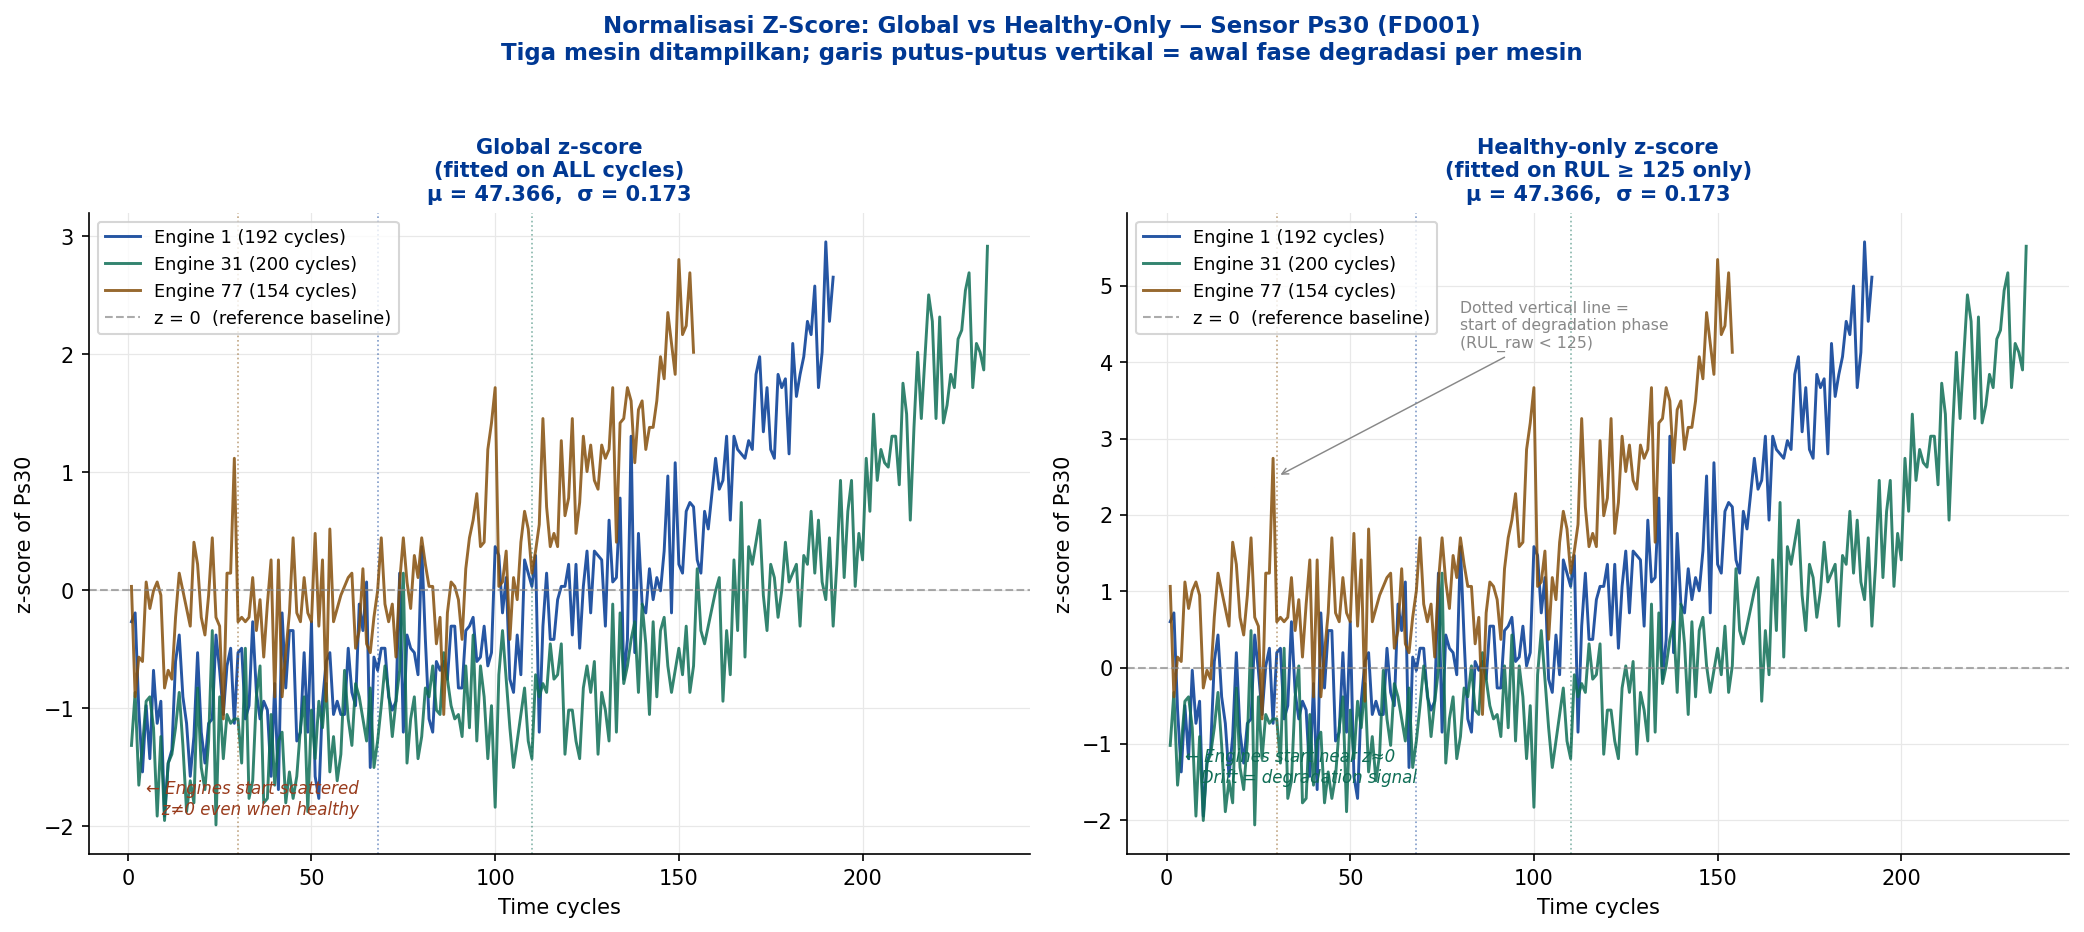
\includegraphics[width=0.96\textwidth]{images/plot_D13_norm_comparison.png}
  \caption{Perbandingan normalisasi global vs \textit{healthy-only}
    untuk sensor Ps30 pada tiga mesin FD001 ---
    kanan: ketiga mesin mulai di $z \approx 0$ dan \textit{drift}
    seiring degradasi}
  \label{fig:norm_comparison}
\end{figure}

% ══════════════════════════════════════════════════════════════════════════════
\section{Seleksi Fitur}

\subsection{Korelasi Pearson Antar Sensor}

\begin{figure}[H]
  \centering
  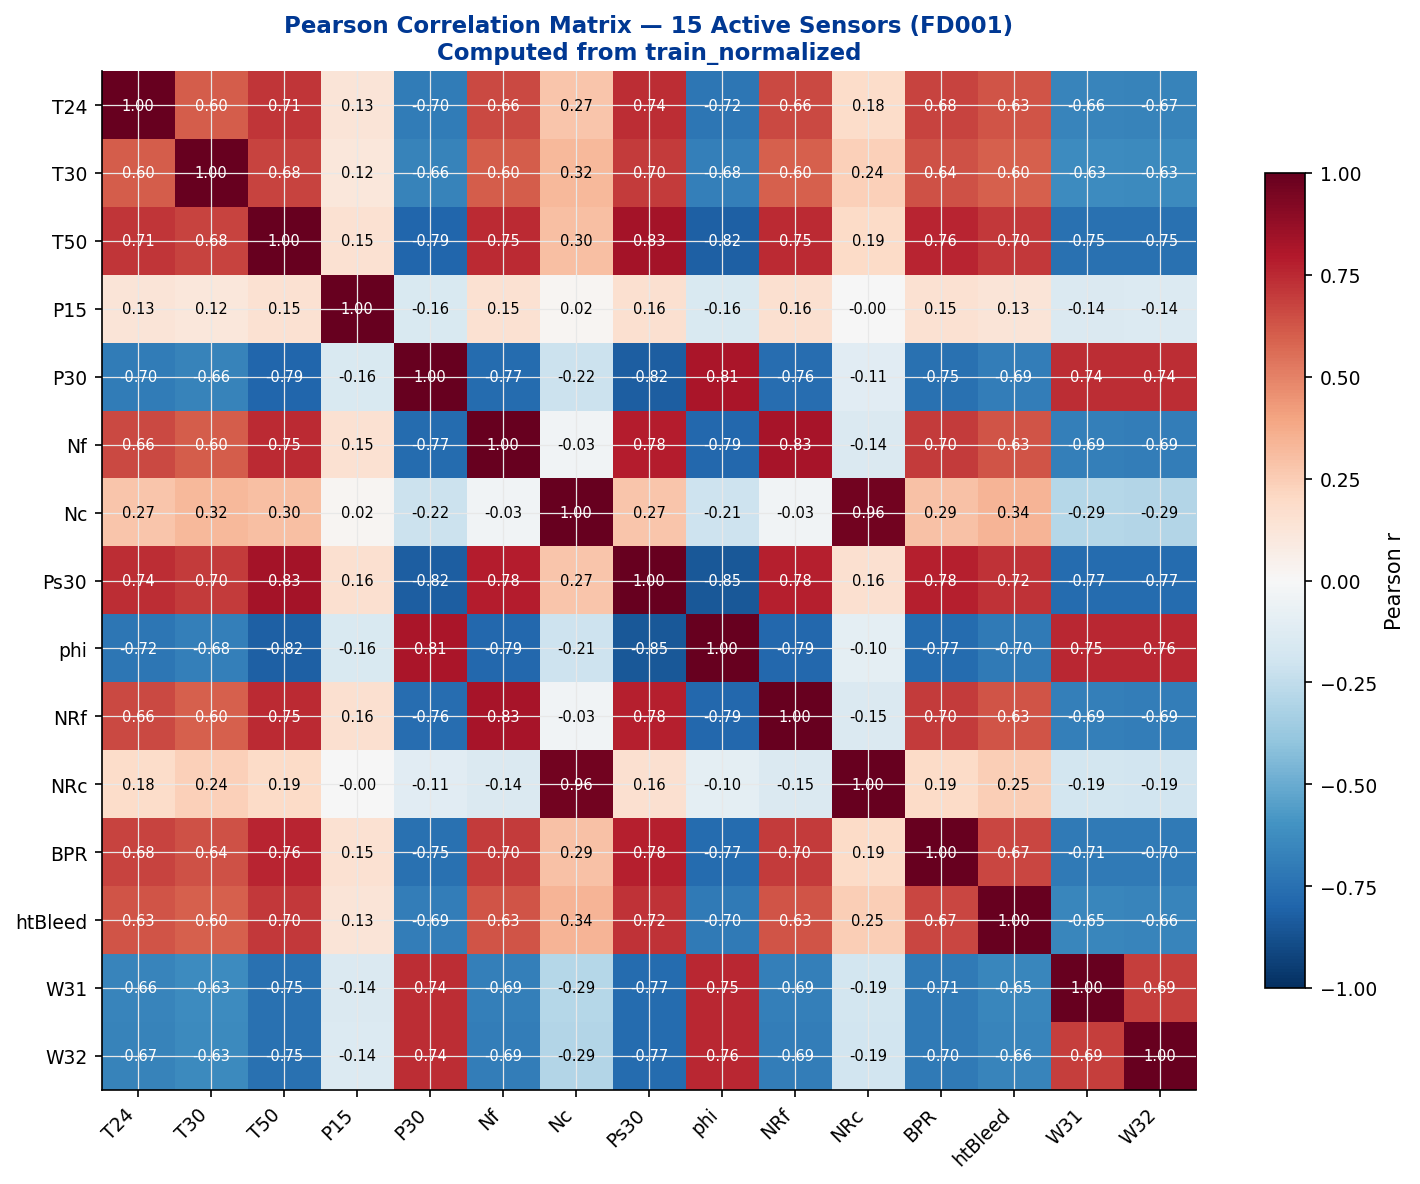
\includegraphics[width=0.82\textwidth]{images/plot_A2_correlation.png}
  \caption{Matriks korelasi Pearson antar 15 sensor aktif FD001 ---
    Nc--NRc ($r = 0{,}96$) dan Nf--NRf ($r = 0{,}83$) menunjukkan
    redundansi tinggi}
  \label{fig:corr}
\end{figure}

\subsection{PCA}

\begin{figure}[H]
  \centering
  \begin{subfigure}[b]{0.48\textwidth}
    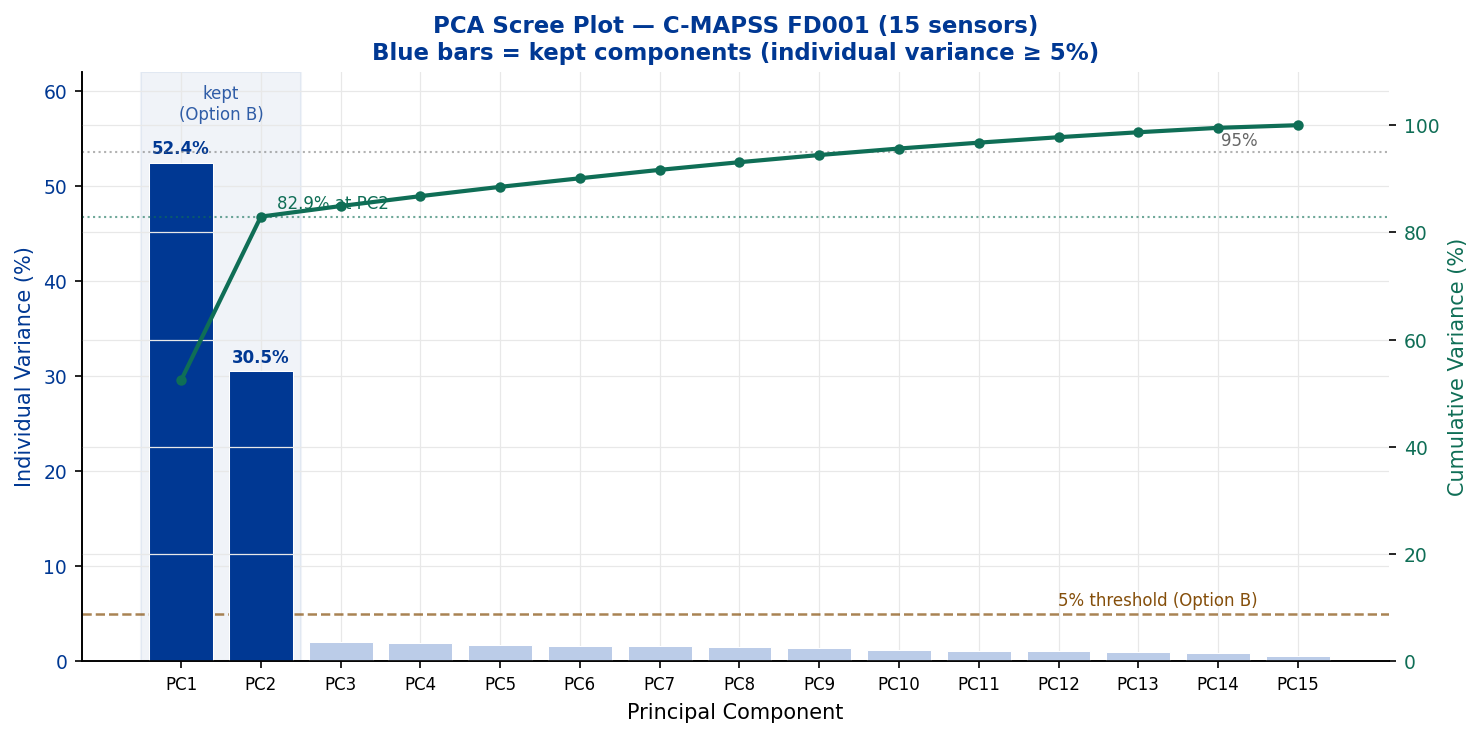
\includegraphics[width=\textwidth]{images/plot_A3_scree.png}
    \caption{Python}
  \end{subfigure}
  \hfill
  \begin{subfigure}[b]{0.48\textwidth}
    
\includegraphics[width=\textwidth]{images/matlab_A3_scree.png}
    \caption{MATLAB}
  \end{subfigure}
  \caption{\textit{Scree plot} PCA FD001 --- \textit{cliff} setelah PC2;
    2 komponen dipertahankan (varians $\geq 5\%$, kumulatif 82,9\%)}
  \label{fig:scree}
\end{figure}

\begin{table}[H]
\centering\small
\caption{Ringkasan PCA per sub-dataset}
\label{tab:pca}
\begin{tabular}{lcccl}
\toprule
Sub-dataset & Sensor & Komponen & Kumulatif & Dominan \\
\midrule
FD001 & 15 & 2 & 82,9\% & PC1: speed (52,4\%), PC2: pressure contrast \\
FD002 & 21 & 4 & 74,8\% & PC1: speed (41,6\%), PC3: epr (8,4\%) \\
FD003 & 16 & 3 & 87,8\% & PC1: speed (60,2\%) \\
FD004 & 21 & 3 & 77,5\% & PC1: speed (48,4\%) \\
\bottomrule
\end{tabular}
\end{table}

\begin{figure}[H]
  \centering
  \begin{subfigure}[b]{0.48\textwidth}
    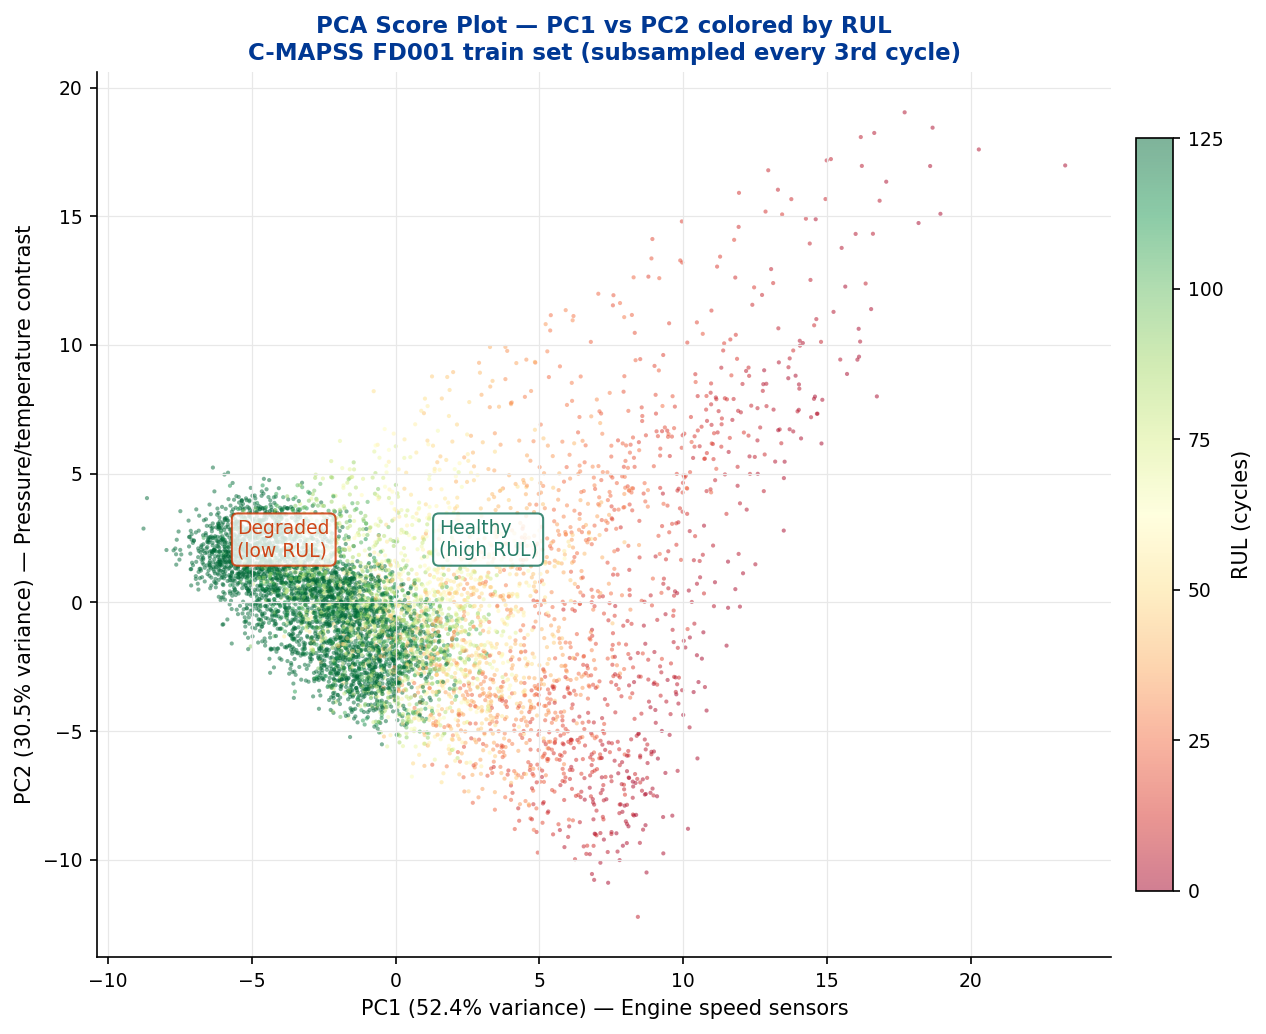
\includegraphics[width=\textwidth]{images/plot_A4_pca_scatter.png}
    \caption{Python}
  \end{subfigure}
  \hfill
  \begin{subfigure}[b]{0.48\textwidth}
    
\includegraphics[width=\textwidth]{images/matlab_A4_pca_scatter.png}
    \caption{MATLAB}
  \end{subfigure}
  \caption{PC1 vs PC2 diwarnai berdasarkan RUL --- hijau = sehat,
    merah = mendekati gagal; pola konsisten antara Python dan MATLAB}
  \label{fig:pca_scatter}
\end{figure}

\subsection{Pipeline Spreadsheet}

\begin{table}[H]
\centering\small
\caption{Evolusi spreadsheet v3--v6}
\label{tab:spreadsheet}
\begin{tabular}{llp{9cm}}
\toprule
Versi & Sheet Baru & Isi \\
\midrule
v3 & train, test, RUL & Data raw + kolom komputasi \\
v4 & train\_normalized & Sensor ternormalisasi \\
v5 & test\_normalized, stats, correlation, engine\_summary
   & Statistik, korelasi, ringkasan mesin \\
v6 & pca\_params, pca\_train, pca\_test & Eigenvectors + skor PC \\
\bottomrule
\end{tabular}
\end{table}

% ══════════════════════════════════════════════════════════════════════════════
\section{Model \textit{Artificial Neural Network}}

\subsection{Arsitektur dan Konfigurasi}

\begin{figure}[H]
  \centering
  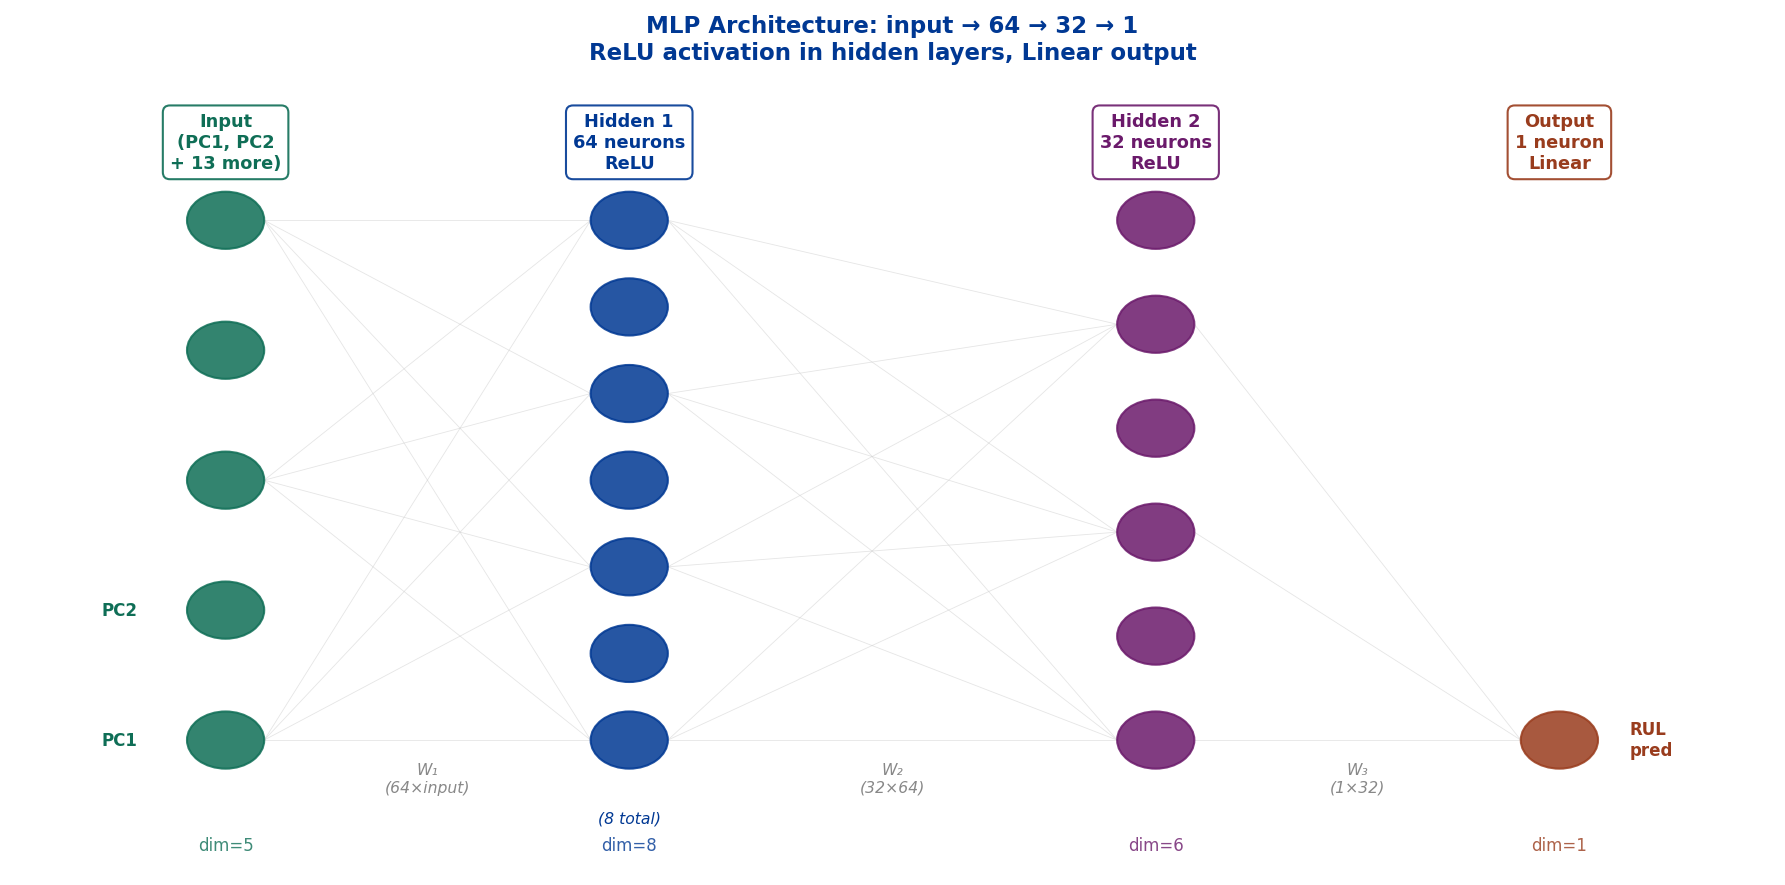
\includegraphics[width=0.88\textwidth]{images/plot_D14_mlp_arch.png}
  \caption{Arsitektur MLP: input $\to$ 64 $\to$ 32 $\to$ 1
    (diagram Python)}
  \label{fig:mlp_arch}
\end{figure}

\begin{figure}[H]
  \centering
  \begin{subfigure}[b]{0.42\textwidth}
    
\includegraphics[width=\textwidth]{images/matlab_arch_pca.png}
    \caption{Model PCA --- Input = 2}
  \end{subfigure}
  \hfill
  \begin{subfigure}[b]{0.42\textwidth}
    
\includegraphics[width=\textwidth]{images/matlab_arch_norm.png}
    \caption{Model NORM --- Input = 15}
  \end{subfigure}
  \caption{Diagram arsitektur jaringan dari MATLAB \texttt{view(net)} ---
    Input $\to$ Hidden1 (64, tansig) $\to$ Hidden2 (32, tansig)
    $\to$ Output (1, purelin)}
  \label{fig:mlp_arch_matlab}
\end{figure}

\begin{table}[H]
\centering\small
\caption{Konfigurasi pelatihan ANN --- Python vs MATLAB}
\label{tab:ann_config}
\begin{tabular}{lll}
\toprule
Parameter & Python (PyTorch) & MATLAB (feedforwardnet) \\
\midrule
Arsitektur   & input $\to$ 64 $\to$ 32 $\to$ 1
             & input $\to$ 64 $\to$ 32 $\to$ 1 \\
Aktivasi     & ReLU + Linear output
             & tansig + purelin output \\
Optimizer    & Adam, lr $= 10^{-3}$
             & trainscg (Scaled Conjugate Gradient) \\
Epoch        & 500 & 500 \\
Batch size   & 512 & full batch \\
Target       & RUL\_capped (125) & RUL\_capped (125) \\
\bottomrule
\end{tabular}
\end{table}

\subsection{Target: RUL Capped}

\begin{figure}[H]
  \centering
  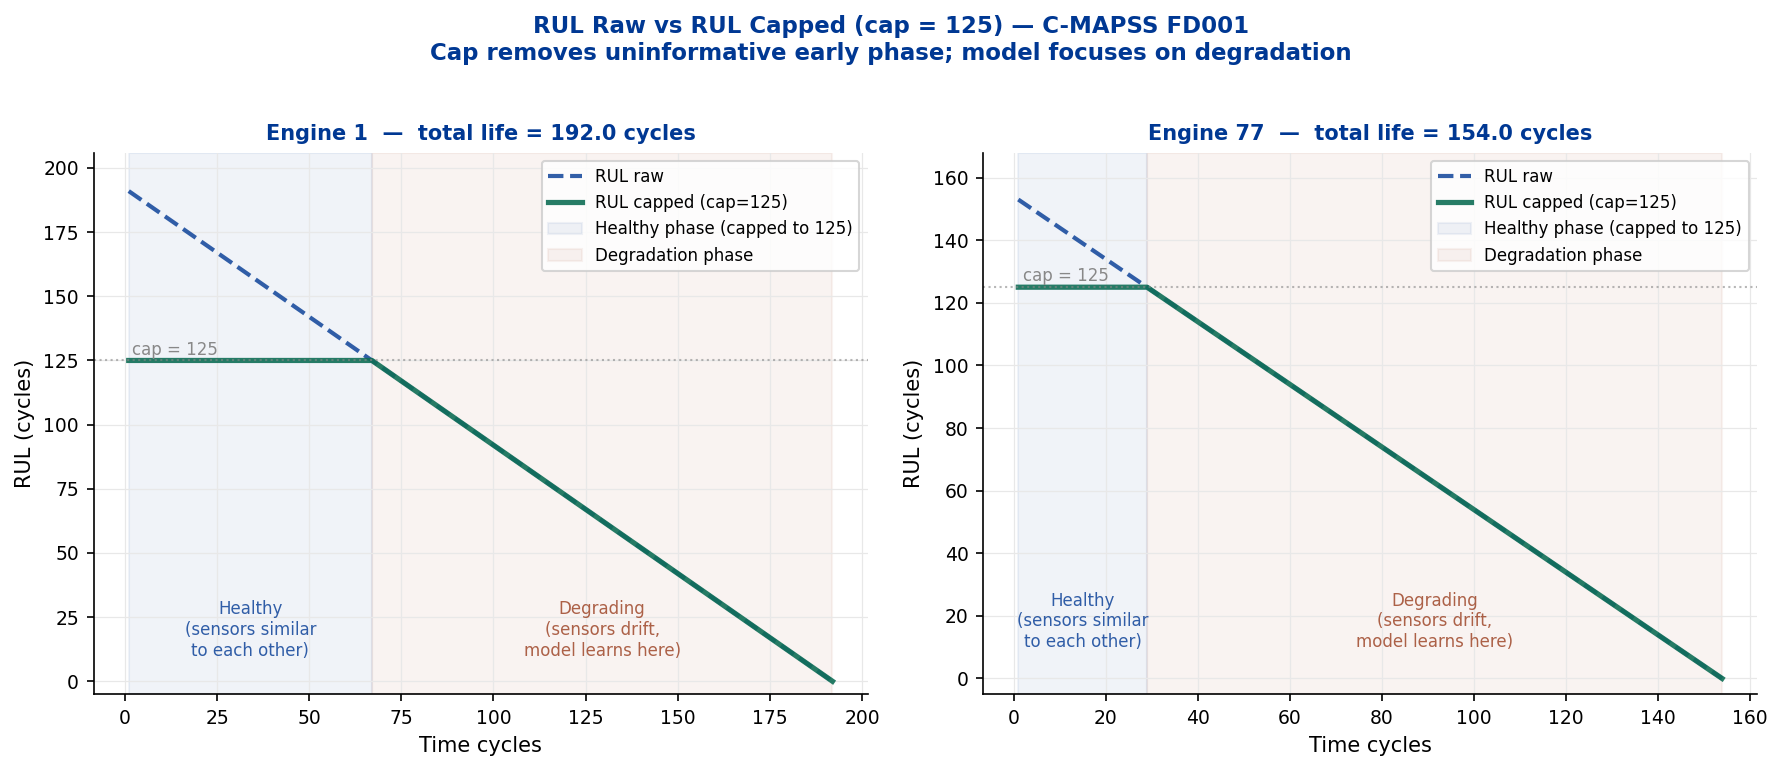
\includegraphics[width=0.88\textwidth]{images/plot_D12_rul_cap.png}
  \caption{RUL raw vs RUL capped (cap $= 125$) untuk dua mesin ---
    fase sehat diratakan, model difokuskan pada fase degradasi}
  \label{fig:rul_cap}
\end{figure}

\subsection{NASA Score}

\begin{figure}[H]
  \centering
  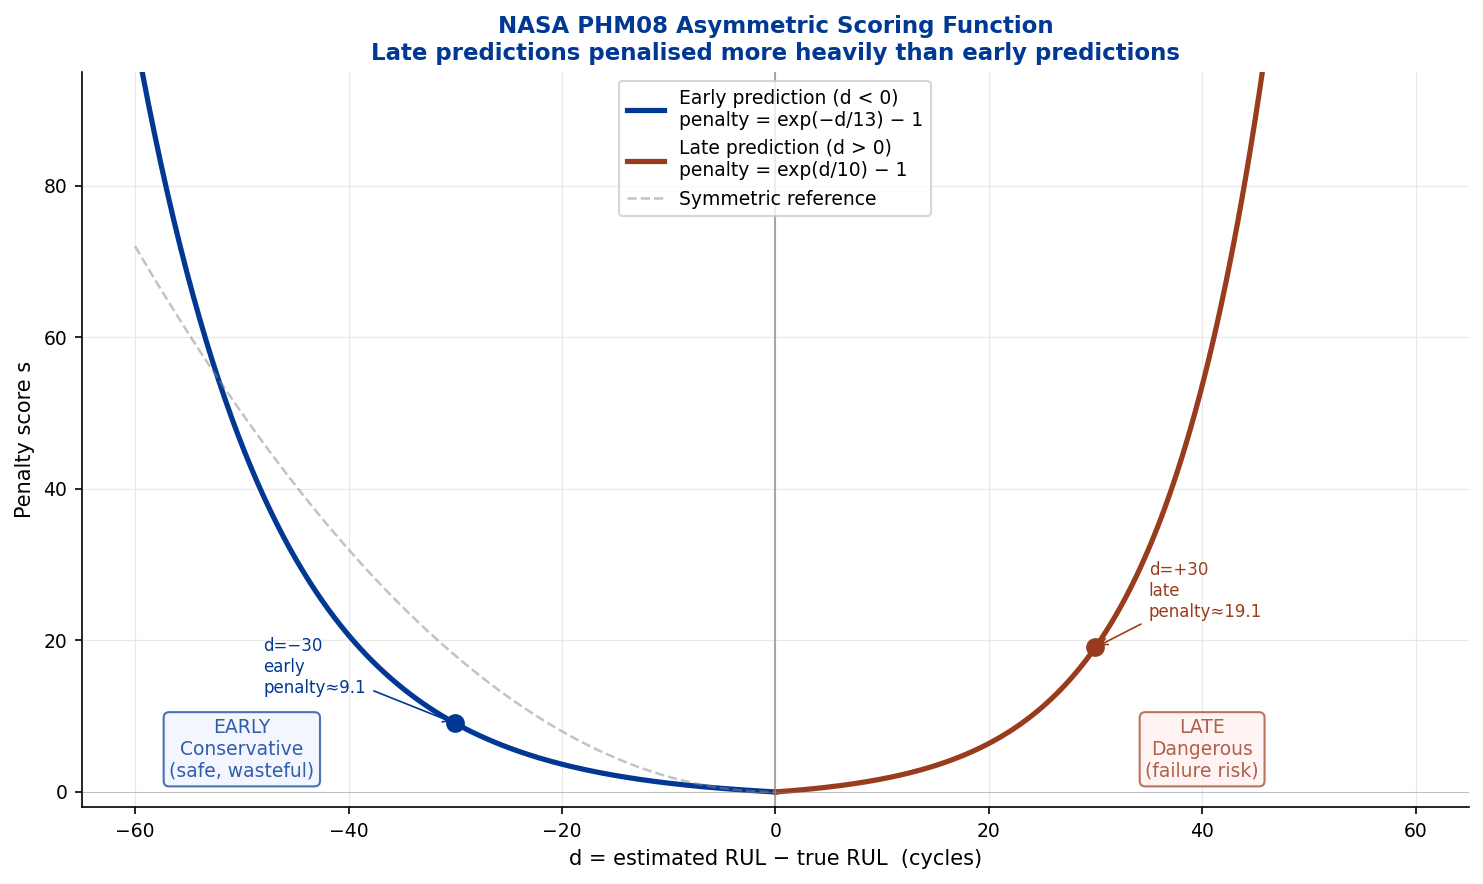
\includegraphics[width=0.72\textwidth]{images/plot_D11_nasa_score.png}
  \caption{Kurva penalti NASA Score --- prediksi \textit{late} ($d > 0$)
    dihukum lebih berat karena membahayakan keselamatan}
  \label{fig:nasa_score}
\end{figure}

\subsection{Hasil Benchmark Python}

\begin{figure}[H]
  \centering
  \begin{subfigure}[b]{0.48\textwidth}
    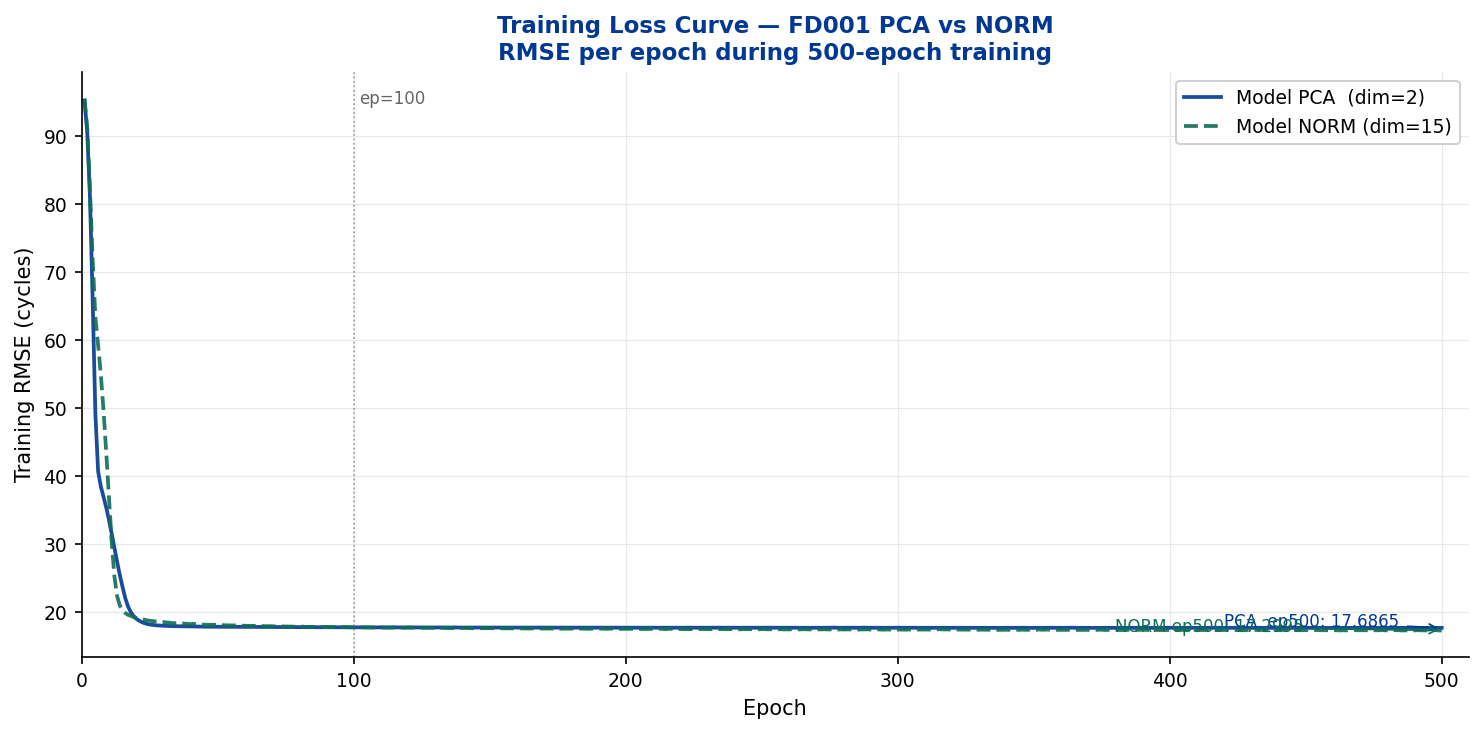
\includegraphics[width=\textwidth]{images/plot_B5_loss_curve.png}
    \caption{Python}
  \end{subfigure}
  \hfill
  \begin{subfigure}[b]{0.48\textwidth}
    
\includegraphics[width=\textwidth]{images/matlab_B5_loss_curve.png}
    \caption{MATLAB}
  \end{subfigure}
  \caption{Kurva \textit{loss} FD001 --- Python Adam konvergen lebih
    cepat; MATLAB trainscg menunjukkan pola konvergensi berbeda}
  \label{fig:loss}
\end{figure}

\begin{table}[H]
\centering\small
\caption{Hasil benchmark Python --- 8 model (4 sub-dataset $\times$ 2 input)}
\label{tab:benchmark_py}
\begin{tabular}{llcrrr}
\toprule
Sub-dataset & Input & Dim & RMSE & MAE & NASA Score \\
\midrule
FD001 & \textbf{PCA}  & 2  & \textbf{17,80} & \textbf{12,55} & \textbf{815} \\
FD001 & NORM & 15 & 18,21 & 13,52 & 929 \\
\midrule
FD002 & \textbf{PCA}  & 4  & \textbf{29,30} & \textbf{20,52} & 14.423 \\
FD002 & NORM & 21 & 29,45 & 20,73 & \textbf{12.990} \\
\midrule
FD003 & PCA  & 3  & 21,87 & 16,17 & 2.650 \\
FD003 & \textbf{NORM} & 16 & \textbf{20,16} & \textbf{15,28} & \textbf{1.783} \\
\midrule
FD004 & PCA  & 3  & 30,59 & 23,28 & 9.267 \\
FD004 & \textbf{NORM} & 21 & \textbf{29,68} & \textbf{22,38} & \textbf{7.157} \\
\bottomrule
\end{tabular}
\end{table}

\begin{figure}[H]
  \centering
  \begin{subfigure}[b]{0.48\textwidth}
    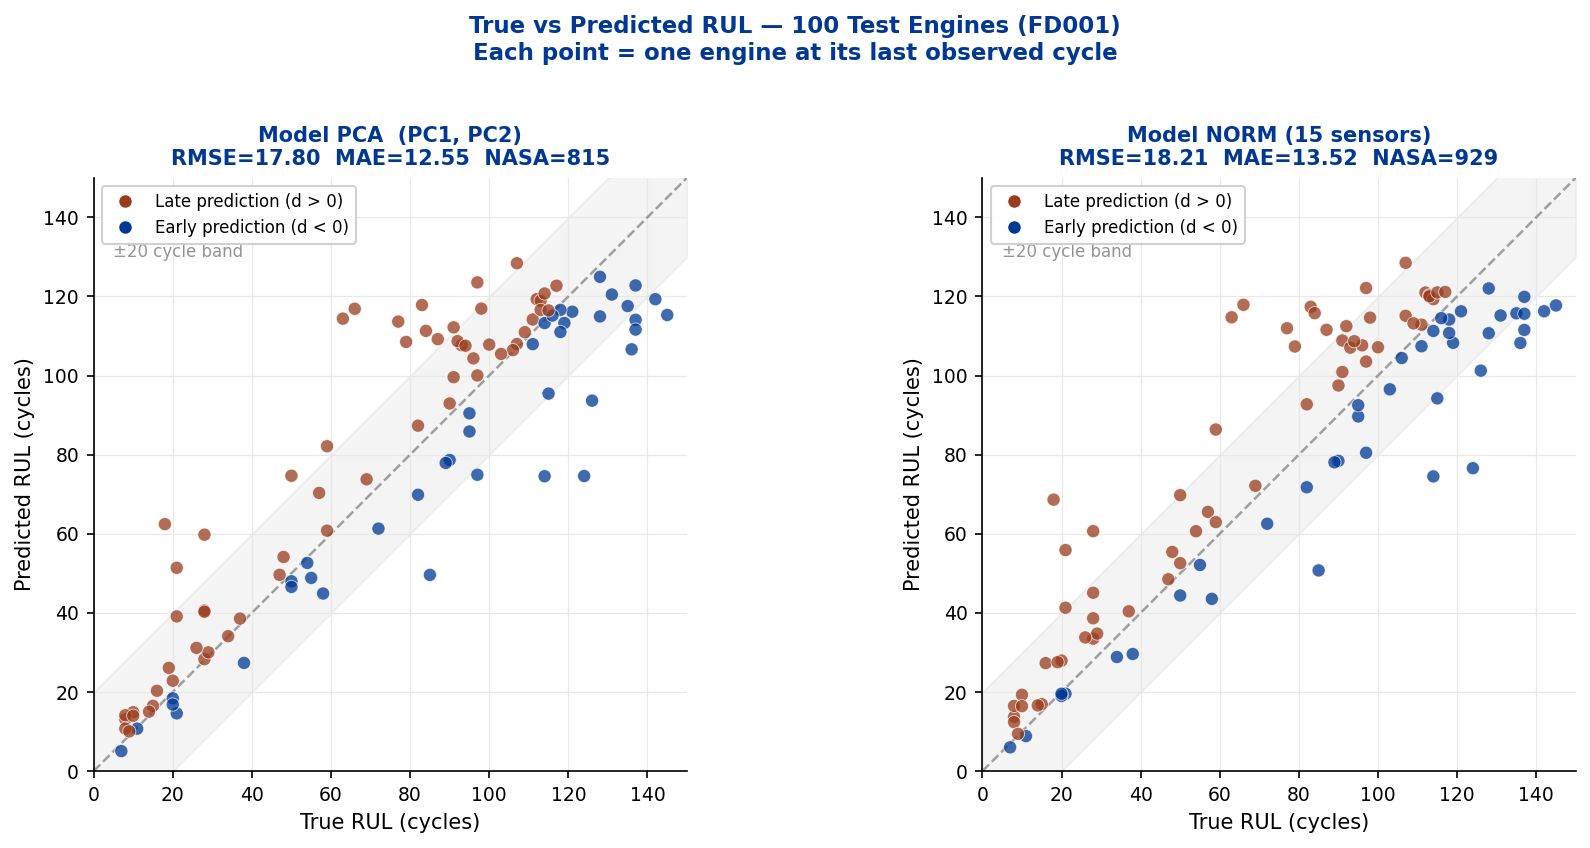
\includegraphics[width=\textwidth]{images/plot_B6_true_vs_pred.png}
    \caption{Python}
  \end{subfigure}
  \hfill
  \begin{subfigure}[b]{0.48\textwidth}
    
\includegraphics[width=\textwidth]{images/matlab_B6_true_vs_pred.png}
    \caption{MATLAB}
  \end{subfigure}
  \caption{True vs Predicted RUL untuk 100 mesin test FD001 ---
    pola diagonal konsisten antara Python dan MATLAB}
  \label{fig:true_pred}
\end{figure}

\begin{figure}[H]
  \centering
  \begin{subfigure}[b]{0.48\textwidth}
    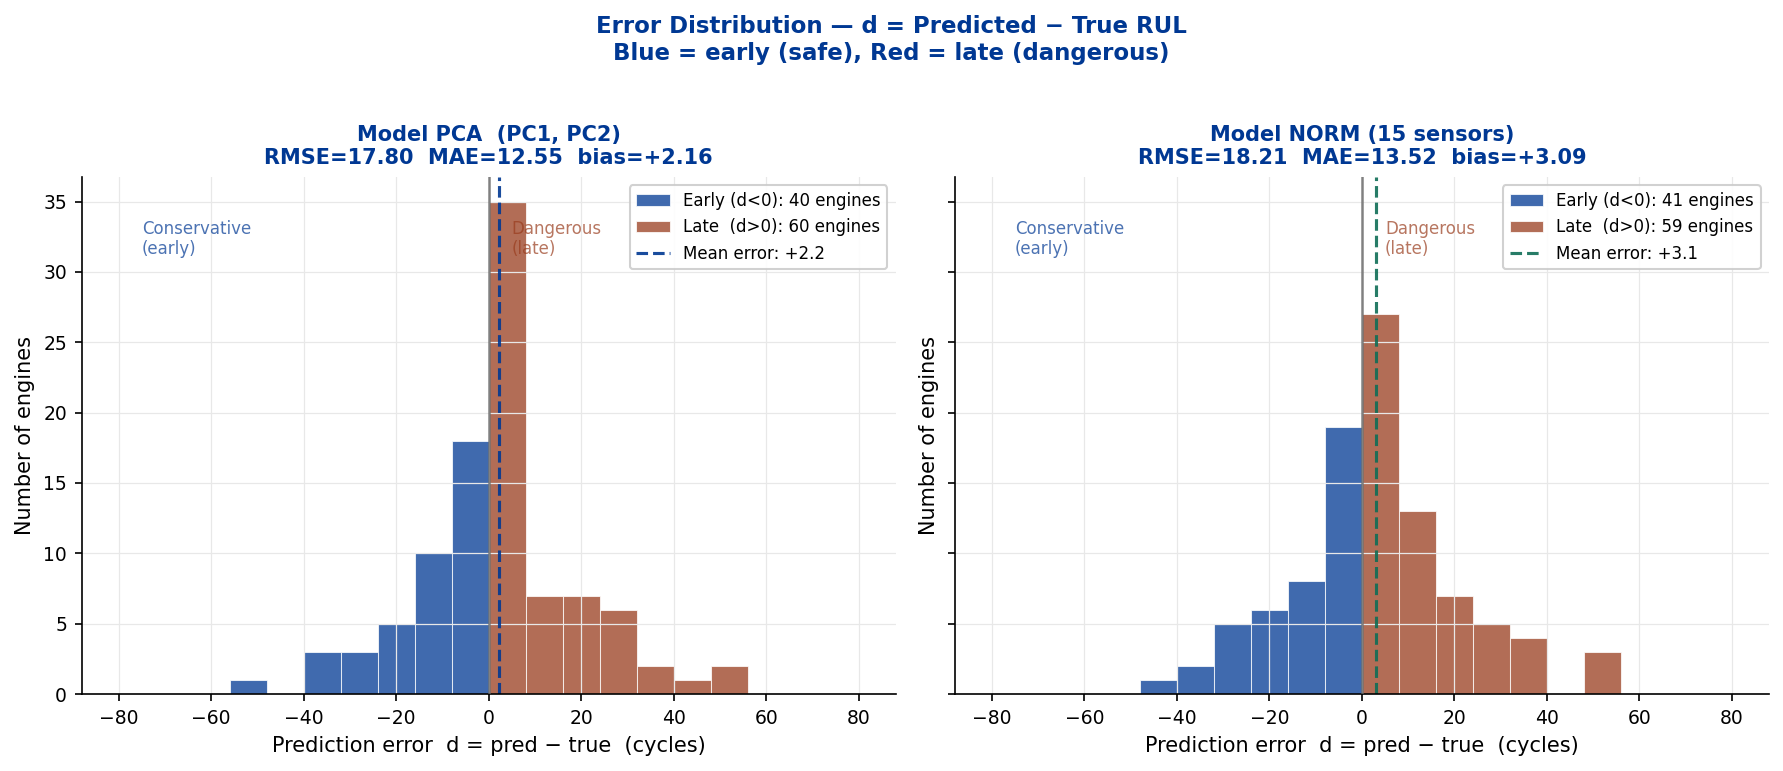
\includegraphics[width=\textwidth]{images/plot_B7_error_dist.png}
    \caption{Python}
  \end{subfigure}
  \hfill
  \begin{subfigure}[b]{0.48\textwidth}
    
\includegraphics[width=\textwidth]{images/matlab_B7_error_dist.png}
    \caption{MATLAB}
  \end{subfigure}
  \caption{Distribusi error prediksi FD001 ---
    distribusi \textit{right-skewed} pada kedua implementasi}
  \label{fig:error_dist}
\end{figure}

\subsection{Analisis Faktor}

\textbf{Faktor 1 --- Kompleksitas sub-dataset} adalah faktor dominan.
Sub-dataset 6 kondisi (FD002, FD004) menghasilkan RMSE $\approx 60\%$
lebih tinggi dari 1 kondisi (FD001, FD003).

\textbf{Faktor 2 --- Tipe input}: PCA lebih baik pada dataset sederhana
(FD001, FD002 berdasarkan RMSE); NORM lebih baik pada dataset kompleks
(FD003, FD004).

% ══════════════════════════════════════════════════════════════════════════════
\section{Analisis Garson}

\subsection{Algoritma}

\begin{align}
  q_1[i,j] &= \frac{|W_1[j,i]|}{\sum_k |W_1[j,k]|} &
  q_2[j,m] &= \frac{|W_2[m,j]|}{\sum_k |W_2[m,k]|} \\[4pt]
  r[i,m]   &= \sum_j q_1[i,j] \cdot q_2[j,m] &
  s[i]     &= \sum_m r[i,m] \cdot |W_3[m]| \\[4pt]
  \text{importance}[i] &= \frac{s[i]}{\sum_k s[k]}
\end{align}

\subsection{Hasil Model PCA}

\begin{figure}[H]
  \centering
  \begin{subfigure}[b]{0.48\textwidth}
    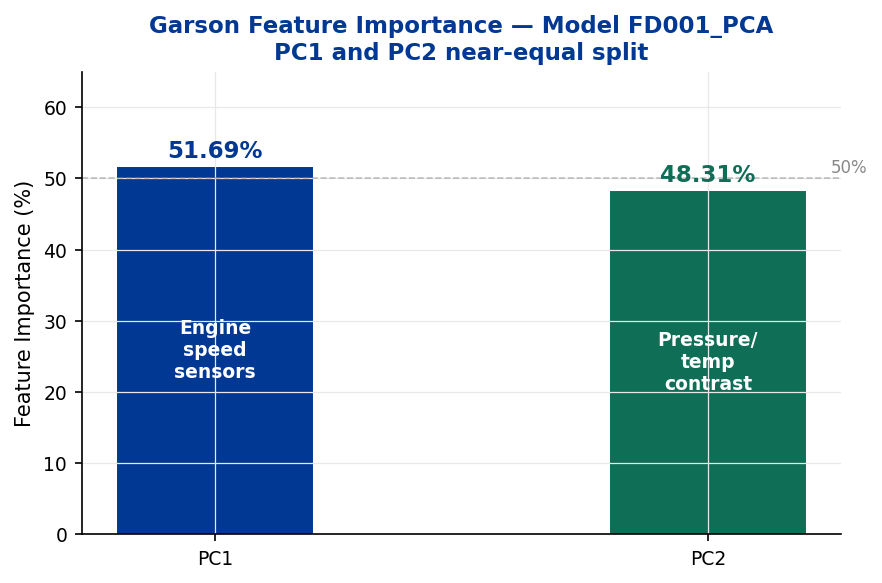
\includegraphics[width=\textwidth]{images/plot_C10_garson_pca.png}
    \caption{Python}
  \end{subfigure}
  \hfill
  \begin{subfigure}[b]{0.48\textwidth}
    
\includegraphics[width=\textwidth]{images/matlab_C10_garson_pca.png}
    \caption{MATLAB}
  \end{subfigure}
  \caption{Garson FD001\_PCA ---
    PC1 dan PC2 hampir seimbang pada kedua implementasi
    (Python: 51,69\%/48,31\% --- MATLAB: 51,08\%/48,92\%)}
  \label{fig:garson_pca}
\end{figure}

\subsection{Hasil Model NORM}

\begin{figure}[H]
  \centering
  \begin{subfigure}[b]{0.48\textwidth}
    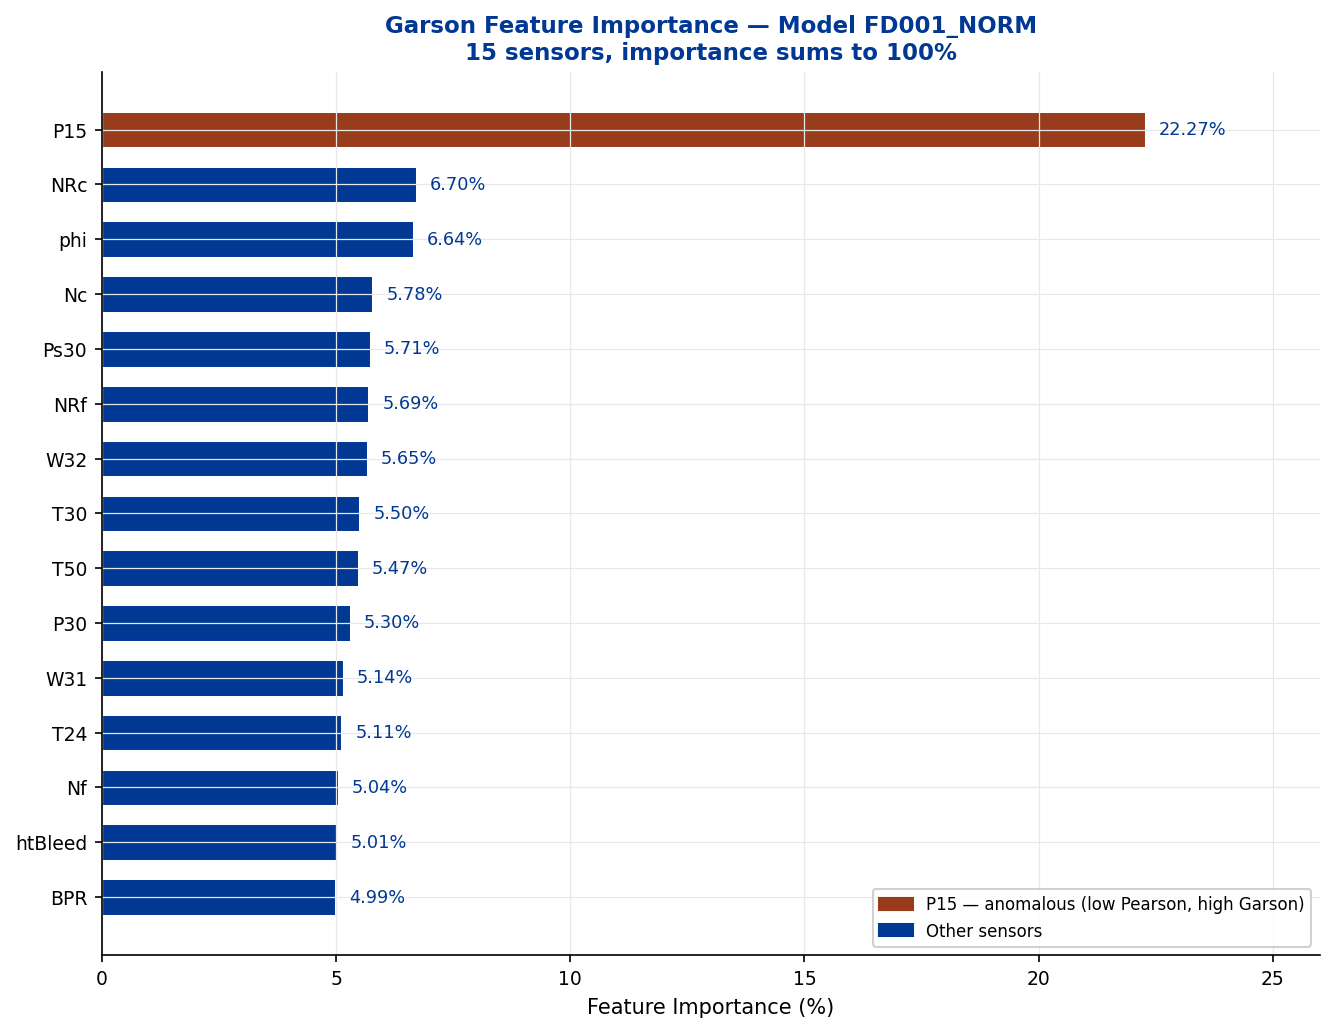
\includegraphics[width=\textwidth]{images/plot_C8_garson_norm.png}
    \caption{Python (ReLU) --- P15 dominan}
  \end{subfigure}
  \hfill
  \begin{subfigure}[b]{0.48\textwidth}
    
\includegraphics[width=\textwidth]{images/matlab_C8_garson_norm.png}
    \caption{MATLAB (tansig) --- distribusi merata}
  \end{subfigure}
  \caption{Garson FD001\_NORM --- perbedaan antara Python (ReLU)
    dan MATLAB (tansig) menunjukkan pengaruh fungsi aktivasi
    terhadap distribusi kepentingan fitur}
  \label{fig:garson_norm}
\end{figure}

\subsection{Perbandingan Tiga Metode}

\begin{figure}[H]
  \centering
  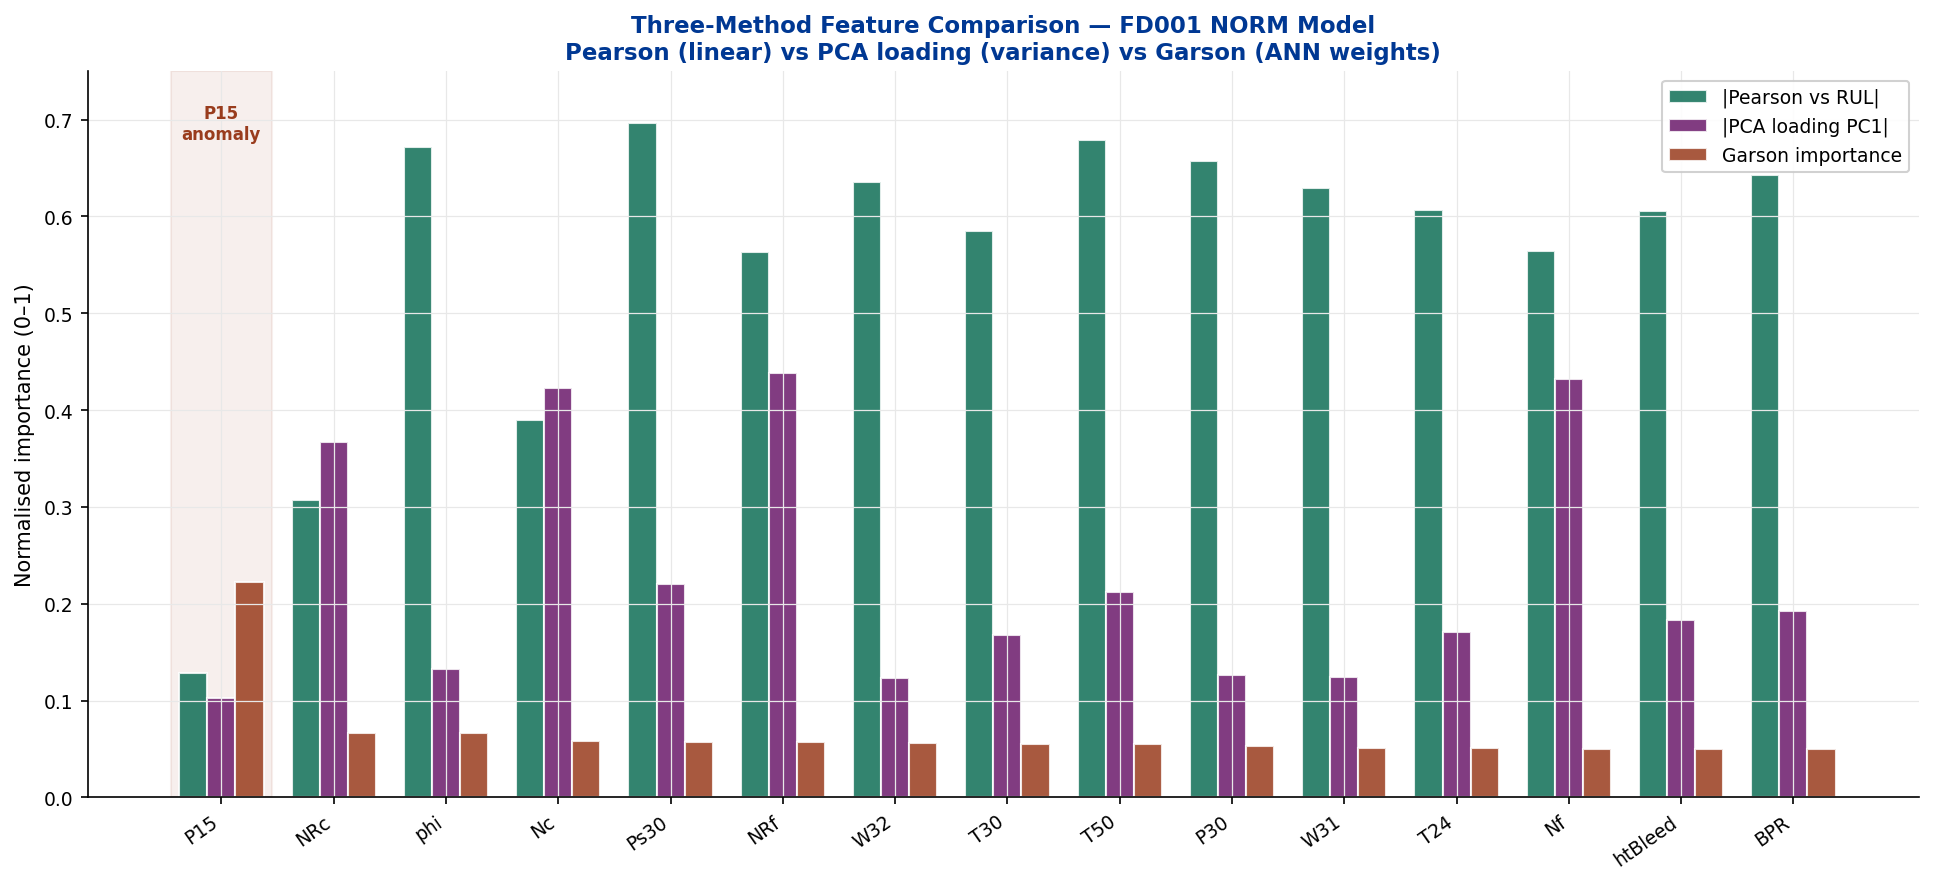
\includegraphics[width=0.95\textwidth]{images/plot_C9_three_method.png}
  \caption{Perbandingan tiga metode seleksi fitur (Python) ---
    anomali P15: Pearson rendah, PCA rendah, Garson tinggi}
  \label{fig:three_method}
\end{figure}

% ══════════════════════════════════════════════════════════════════════════════
\section{Perbandingan Python vs MATLAB}

\subsection{Hasil FD001}

\begin{table}[H]
\centering\small
\caption{Perbandingan hasil FD001 --- Python (PyTorch/Adam/ReLU)
  vs MATLAB (feedforwardnet/trainscg/tansig)}
\label{tab:compare}
\begin{tabular}{llcrrr}
\toprule
Implementasi & Model & Dim & RMSE & MAE & NASA \\
\midrule
\textcolor{uiblue}{Python}
  & PCA  & 2  & \textbf{17,80} & \textbf{12,55} & \textbf{815} \\
\textcolor{uiblue}{Python}
  & NORM & 15 & 18,21 & 13,52 & 929 \\
\midrule
\textcolor{matgreen}{MATLAB}
  & PCA  & 2  & 18,30 & 13,34 & 845 \\
\textcolor{matgreen}{MATLAB}
  & NORM & 15 & 20,91 & 15,75 & 1.319 \\
\bottomrule
\end{tabular}
\end{table}

\subsection{Analisis Perbedaan}

\textbf{Model PCA --- hampir identik}:
Python RMSE 17,80 vs MATLAB 18,30 (selisih 0,50 siklus = 2,8\%).
Kedua implementasi menghasilkan hasil yang konsisten.
Garson PCA juga konsisten: PC1 $\approx$51\%, PC2 $\approx$49\%
pada keduanya.

\textbf{Model NORM --- perbedaan lebih besar}:
Python RMSE 18,21 vs MATLAB 20,91 (selisih 2,70 siklus = 14,8\%).
Perbedaan ini disebabkan oleh:
\begin{enumerate}[noitemsep]
  \item \textbf{Fungsi aktivasi}: Python menggunakan ReLU
    (\textit{piecewise linear}), MATLAB menggunakan tansig
    (\textit{smooth sigmoid}). ReLU lebih efektif menangkap
    hubungan non-linear pada dataset ini.
  \item \textbf{Optimizer}: Adam (Python) vs trainscg (MATLAB).
    Adam dengan \textit{momentum} umumnya menghasilkan konvergensi
    lebih baik untuk dataset ini.
  \item \textbf{Batch training}: Python menggunakan mini-batch 512,
    MATLAB menggunakan full batch --- perbedaan gradient estimation.
\end{enumerate}

\textbf{Implikasi Garson}:
Python menemukan P15 sebagai fitur terpenting (22,27\%) karena
ReLU dapat mengeksploitasi hubungan non-linear tajam. MATLAB
dengan tansig mendistribusikan kepentingan lebih merata ---
Nc (9,92\%) menjadi sensor teratas tanpa dominasi ekstrem.
Keduanya valid; mereka mencerminkan konfigurasi model yang berbeda.

% ══════════════════════════════════════════════════════════════════════════════
\section{Keterbatasan dan Pengembangan}

\begin{enumerate}[noitemsep]
  \item \textbf{MLP tidak memanfaatkan urutan temporal} ---
    LSTM/GRU lebih tepat untuk data \textit{time series}
  \item \textbf{Dataset simulasi} --- degradasi mesin nyata lebih kompleks
  \item \textbf{MATLAB trainscg} menghasilkan RMSE lebih tinggi dari
    Python Adam untuk model NORM --- GPU tidak dimanfaatkan oleh
    \texttt{feedforwardnet}
  \item \textbf{Garson untuk dua lapisan tersembunyi} kurang didukung
    literatur dibandingkan versi satu lapisan
\end{enumerate}

% ══════════════════════════════════════════════════════════════════════════════
\section{Kesimpulan}

\begin{enumerate}[noitemsep]
  \item \textbf{Kompleksitas kondisi operasi adalah faktor dominan}.
    Sub-dataset 6 kondisi menghasilkan RMSE $\approx 60\%$ lebih tinggi
    dari 1 kondisi, terlepas dari implementasi.

  \item \textbf{Tipe input optimal bergantung pada kompleksitas}:
    PCA lebih baik untuk dataset sederhana; NORM lebih baik untuk
    dataset kompleks.

  \item \textbf{Python (Adam/ReLU) menghasilkan RMSE lebih rendah}
    dari MATLAB (trainscg/tansig), terutama untuk model NORM.
    Model PCA hampir identik antara kedua implementasi
    (selisih $< 3\%$).

  \item \textbf{Garson mengungkap pengaruh fungsi aktivasi}:
    ReLU (Python) memusatkan kepentingan pada P15 (22,27\%);
    tansig (MATLAB) mendistribusikan lebih merata.

  \item \textbf{Eliminasi sensor harus per sub-dataset}:
    sensor konstan di FD001 menjadi aktif di FD002.
\end{enumerate}

% ── References ────────────────────────────────────────────────────────────────
\begin{thebibliography}{9}
\bibitem{saxena2008}
  A. Saxena, K. Goebel, D. Simon, N. Eklund,
  ``Damage Propagation Modeling for Aircraft Engine Run-to-Failure Simulation,''
  \textit{Proc.\ 1st Int.\ Conf.\ Prognostics and Health Management (PHM08)},
  Denver, CO, 2008.

\bibitem{garson1991}
  G.D. Garson,
  ``Interpreting Neural Network Connection Weights,''
  \textit{AI Expert}, vol.~6, no.~4, pp.~46--51, 1991.
\end{thebibliography}

\end{document}
